\documentclass[]{article}
\usepackage[utf8]{inputenc}
\usepackage[pdftex]{graphicx} % for includegraphics
\usepackage[bf,font={small,sl}]{caption} % for pretty captions
\usepackage{natbib} % for the bibliography

\title{\texttt{moveHMM}\\ An R package for animal movement modelling}
\author{Michelot T., Langrock R., Patterson T., and Rexstad E.}

\begin{document}
\maketitle

\section*{Introduction}
Animal movement data is growing rapidly, due to the substantial improvement of telemetry technologies. As a result, statistical methods used to analyse this data are brought to their computational limit.

Novel models have been developed in the last decade to reduce the computational cost of statistical inference in movement ecology. In particular, hidden Markov models are increasingly popular in this field, due to their flexibility, and to the efficient algorithms that they offer, see \cite{patterson2009} and \cite{langrock2012}.\\

\texttt{moveHMM} is an R package which implements hidden Markov models (HMMs) for animal movement. A special attention was paid to performance, and the fitting algorithm is implemented in C++ to make it significantly faster.

The goal of this vignette is to give a global overview of the possibilities offered by the package, and to demonstrate its use on a detailed example.

\section{Package features}
In this section, we describe different features included in \texttt{moveHMM}. We describe the global structure of the package, and then describe in more detail the main functions required to fit a HMM to movement data. In particular, we introduce the different options that the functions offer, and explain how the functions' arguments should be chosen.

\subsection{Structure}
The package is articulated around two S3 classes : \texttt{moveData} and \texttt{moveHMM}. The first one is a data frame of the data, essentially gathering time series of the movement metrics of interest, namely the step lengths and turning angles, as well as the covariate values. A \texttt{moveHMM} object is a fitted model, which stores in particular the values of the MLE of the parameters.\\

In order to create a \texttt{moveData} object, the function \texttt{prepData} is called on the tracking data (track points coordinates). Then, the function \texttt{fitHMM} is called on the \texttt{moveData}, and returns a \texttt{moveHMM}.

Both classes can be used through their methods, e.g. \texttt{plot.moveData}, \texttt{decode.moveHMM}, \texttt{AIC.moveHMM}... All the functions are described in more detail in Section \ref{main_functions}, and their use is explained on an example in Section \ref{application}.\\

Figure \ref{struct} illustrates the links between the main components of the package.

\begin{figure}[h]
	\centering
	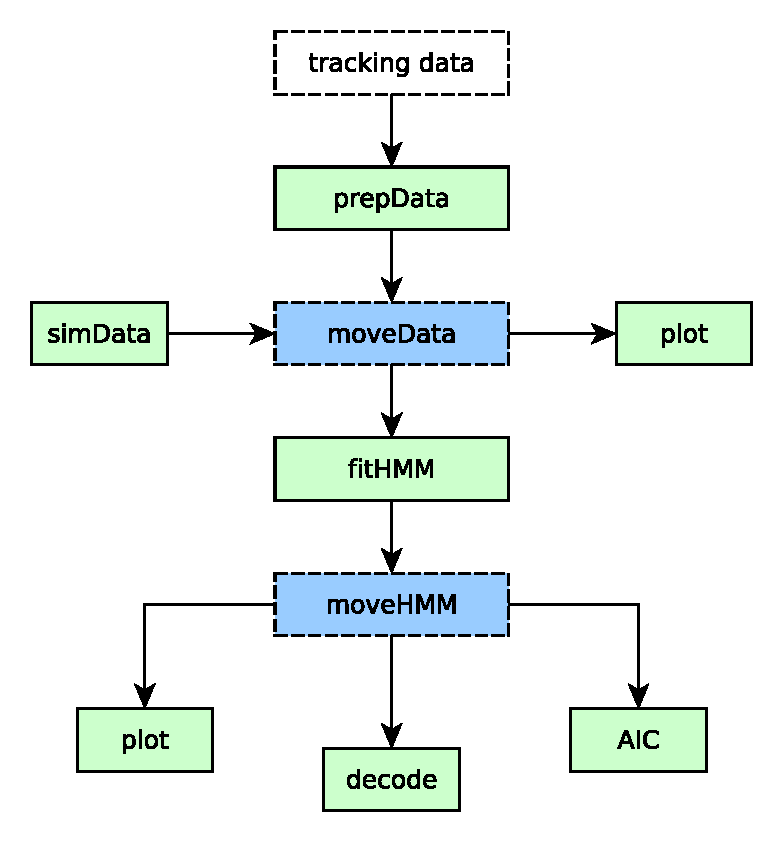
\includegraphics[width=0.5\textwidth]{pictures/struct}
	\caption{Structure of the main components of the package. The blue boxes are S3 classes, and the green boxes are functions. The arrows indicate input and output of data.}
	\label{struct}
\end{figure}


\subsection{Main functions} \label{main_functions}

\subsubsection{prepData}
Most of the time, tracking data consists in time series of either easting-northing coordinates or longitude-latitude values. However, the data needed to use hidden Markov modelling are the time series of step lengths and turning angles.\\

The function \texttt{prepData} computes the steps/angles from the coordinates. As an input, this function takes an R data frame with mandatory column names ``x'' (either easting or longitude) and ``y'' (either northing or latitude). If several animals were observed, there should also be a colum ``ID'' which identifies the animal being observed. If there is no ``ID'' column, all observations will be considered to concern a single animal. All additional columns are considered as covariates.

In addition to the data frame, \texttt{prepData} takes an argument \texttt{type}, which can either be ``GCD'' (default) or ``euclidean''. The former indicates that the coordinates are longitude-latitude values, and the latter that they are easting-northing values. This option is used in the computation of the step lengths.\\

\texttt{prepData} outputs a data frame, with the same columns as the input, plus columns ``step'' and ``angle''. This object is of the class \texttt{moveData}, and can be plotted using the generic method \texttt{plot}.

\subsubsection{fitHMM}
To an object \texttt{moveData} can then be fitted an HMM, using the function \texttt{fitHMM}. This function takes the following arguments :

\begin{itemize}
	\item \texttt{data} : a \texttt{moveData} object.
	\item \texttt{nbStates} : the number of states of the HMM to be fitted.
	\item \texttt{stepPar0} : initial values for the step length distribution parameters. Note that they should be in a vector, in the order expected by the density function of the used distribution (except for ``gamma'' which expects mean and standard deviation, in this order, instead of shape and rate). For an example, see Section \ref{application}.
	\item \texttt{anglePar0} : initial values for the turning angle distribution parameters. Same remark as for \texttt{stepPar0}. Can be \texttt{NULL} if the angle distribution is not estimated.
	\item \texttt{beta0} : initial values for the regression coefficients of the transition probabilities. If set to \texttt{NULL}, a default value is chosen such that the transition probabilities do not depend on the covariates, and diagonal elements of the transition probability matrix are dominant.
	\item \texttt{delta0} : initial value for the initial distribution of the HMM. If set to \texttt{NULL}, the default value is chosen to be \texttt{rep(1/nbStates,nbStates)}.
	\item \texttt{formula} : the formula that determines the relationship between the transition probabilities and the covariates. Default is \texttt{~1}, i.e. covariate-free model.
	\item \texttt{stepDist} : distribution for the step lengths. Possible values are ``gamma'' (default), ``weibull'', ``lnorm'', and ``exp''.
	\item \texttt{angleDist} : distribution for the turning angles. Possible values are ``vm'' (Von Mises distribution, default), ``wrpcauchy'', and ``none'' (only steps should be modelled).
	\item \texttt{angleMean} : mean parameter of the angle distribution. If set to \texttt{NULL}, the angle mean is estimated.
	\item \texttt{zeroInflation} : boolean value, \texttt{TRUE} if zero-inflation should be included in the model, \texttt{FALSE} otherwise (default).
	\item \texttt{stationary} : boolean value, \texttt{TRUE} if the initial distribution is considered to be the stationary distribution, \texttt{FALSE} otherwise (default).
	\item \texttt{verbose} : level of printing of the optimization function. Can be \texttt{0} (no printing), \texttt{1} (first and last iteration of the optimization are printed), or \texttt{2} (all iterations are printed).
\end{itemize}

This function outputs a list of information about the model. Most elements of that list are only meant to be used by the \texttt{moveHMM} methods (see Section \ref{methods}), but a few can be informative \textit{per se} :
\begin{itemize}
	\item \texttt{mle} contains the estimates of the parameters of the model;
	\item \texttt{mod} contains the output of the optimization function \texttt{nlm}, including \texttt{mod\$minimum} (minimum of the negative log-likelihood) and \texttt{mod\$hessian}, the hessian of the negative log-likelihood function at its minimum.
	\item \texttt{states} contains the sequence of most probable states, as computed by the Viterbi algorithm.
\end{itemize}

\subsubsection{Classes methods} \label{methods}
Methods (i.e. class functions) are available for both \texttt{moveData} and \texttt{moveHMM} objects, to operate on them. Here is a list of them ; for details on the options, see the documentation, and for an example of their use, see Section \ref{application}.

\begin{itemize}
	\item \texttt{plot.moveData} plots a few graphs to illustrate the data : a map of each animal's track, time series of the steps and angles, histograms of the steps and angles.
	\item \texttt{plot.moveHMM} plots a few graphs to illustrate the fitted model : a map of each animal's track, colored by states, plots of the estimated density functions, plots of the transition probabilities as functions of the covariates.
	\item \texttt{AIC.moveHMM} returns the AIC of the fitted model.
	\item \texttt{pseudoRes.moveHMM} computes the pseudo-residuals of the model.
	\item \texttt{stateProbs.moveHMM} computes the state probabilities for each observation.
	\item \texttt{decode.moveHMM} wraps \texttt{pseudoRes} and \texttt{stateProbs}.
	\item \texttt{confIntervals.moveHMM} computes the confidence intervals for the step length distribution parameters and for the regression coefficients of the transition probabilities.
	\item \texttt{deltaMethod.moveHMM} computes the confidence intervals for the turning angle distribution parameters, using the delta method.
\end{itemize} 

\subsubsection{simData}
The function \texttt{simData} simulates movement data from an HMM, given its parameters. The returned object is of the class \texttt{moveData}, and can then be visualized using \texttt{plot.moveData}, or fitted using \texttt{fitHMM}.\\

In order to simulate data, the following arguments can be provided :
\begin{itemize}
	\item \texttt{nbAnimals} : number of animals;
	\item \texttt{nbStates} : number of states of the HMM from which the data is simulated;
	\item \texttt{stepDist} : distribution of the simulated step lengths. Possible values are ``gamma'' (default), ``weibull'', ``lnorm'', and ``exp''.
	\item \texttt{angleDist} : distribution of the simulated turning angles. Possible values are ``vm'' (Von Mises distribution, default), ``wrpcauchy'', and ``none'' (only steps should be simulated).
	\item \texttt{stepPar} :  parameters of the step distribution. Note that they should be in a vector, in the order expected by the density function of the used distribution (except for ``gamma'' which expects mean and standard deviation, in this order, instead of shape and rate). For an example, see Section \ref{application}.
	\item \texttt{anglePar} : parameters of the angle distribution. Same remark as for \texttt{stepPar}. Can be \texttt{NULL} if angles are not simulated.
	\item \texttt{beta} : matrix of regression coefficients for the transition probabilities. If not specified, random values are chosen.
	\item \texttt{nbCovs} : number of covariates to simulate.
	\item \texttt{zeroInflation} : \texttt{TRUE} if zero-inflation should be included in the simulation, \texttt{FALSE} otherwise (default).
	\item \texttt{obsPerAnimal} : range of the number of observations to be simulated for each animal, as \texttt{c(nbMin,nbMax)}. Default : \texttt{c(500,1500)}.
\end{itemize}

\section{Application} \label{application}
We take the user through a detailed example. I think that we will include a (relatively small) real data set in \texttt{data/}, which will serve in this example.

\subsection{Movement data}
We describe the format of the data that the user needs to input :
\begin{itemize}
	\item R data frame;
	\item regular time intervals;
	\item mandatory column names : "ID", "x", "y", ...;
	\item additional columns are considered as covariates;
	\item warn the user about missing covariate values;
	\item warn the user about outliers.
\end{itemize}

We explain how to use the function \texttt{prepData} to transform the tracking data into movement data.

We explain how to use \texttt{plot.moveData}, which graphical options are available, and we display the output.

\subsection{Fitting the model}
We go through all the options of \texttt{fitHMM}, and demonstrate its use on the real data example.

Here we can warn the user about the choice of the initial values.

\subsection{Using the model}
We need to mention :
\begin{itemize}
	\item Plotting : describe the function \texttt{plot.moveHMM} and the graphical options, and display all the plots;
	\item Decoding : describe the decoding functions, such as \texttt{viterbi}, \texttt{stateProbs}, and \texttt{pseudoRes}, and apply them to the data;
	\item Assessing : we don't really have the functions yet, but we will need to explain how to obtain confidence intervals, and how to plot them. We might want to mention the simulation function as an assessing tool.
\end{itemize}


\begin{thebibliography}{}

\bibitem[\protect\citeauthoryear{Langrock}{2012}]{langrock2012}
\textsc{Langrock R., King R., Matthiopoulos J., Thomas L., Fortin D., Morales J.M.} (2012),
``Flexible and practical modeling of animal telemetry data: hidden Markov models and extensions''
\textit{Ecology}, 93 (11), 2336-2342.

\bibitem[\protect\citeauthoryear{Patterson}{2009}]{patterson2009}
\textsc{Patterson T.A., Basson M., Bravington M.V., Gunn J.S.} (2012),
``Classifying movement behaviour in relation to environmental conditions using hidden Markov models''
\textit{Journal of Animal Ecology}, 78 (6), 1113-1123.

\end{thebibliography}

\end{document}